\documentclass[11pt,a4paper]{article}

% Packages
\usepackage[utf8]{inputenc}
\usepackage[T1]{fontenc}
\usepackage{amsmath,amssymb,amsthm}
\usepackage{mathtools}
\usepackage{geometry}
\geometry{margin=2.5cm}
\usepackage{graphicx}
\usepackage{hyperref}
\usepackage{cleveref}
\usepackage{algorithm}
\usepackage{algorithmic}
\usepackage{booktabs}
\usepackage{caption}
\usepackage{subcaption}
\usepackage{natbib}
\bibliographystyle{plainnat}

% Theorem environments
\newtheorem{theorem}{Theorem}
\newtheorem{proposition}[theorem]{Proposition}
\newtheorem{lemma}[theorem]{Lemma}
\newtheorem{remark}[theorem]{Remark}
\newtheorem{definition}[theorem]{Definition}

% Notation shortcuts
\newcommand{\E}{\mathbb{E}}
\newcommand{\R}{\mathbb{R}}
\newcommand{\dd}{\mathrm{d}}
\newcommand{\mup}{\mu_t}

\title{Deep Mean-Field BSDE Methods for Optimal Market-Making\\in Limit Order Books}

\author{
  Christian Garry \\
  Department of Mathematical Sciences \\
  Durham University \\
  \texttt{christian.garry@durham.ac.uk}
}

\date{April 2026}

\begin{document}
\maketitle

% ============================================================
\begin{abstract}
We present a deep learning solver for optimal market-making in limit order books, combining the Deep BSDE method of Han, Jentzen, and E~(2018) with the McKean--Vlasov fictitious play framework of Han, Hu, and Long~(2022). Starting from the multi-dealer intensity control game of Cont and Xiong~(2024), we derive two computational formulations: (i)~a continuous inventory relaxation where the Poisson order flow is approximated by a diffusion, yielding a standard MV-FBSDE amenable to the Deep BSDE architecture; and (ii)~an exact jump-diffusion formulation (FBSDEJ) where the neural network outputs both the Brownian gradient $Z_t$ and the Poisson jump controls $U_t^\pm$. In both cases, optimal bid-ask quotes emerge directly from the learned gradient process via the HJB first-order condition, recovering the classical Avellaneda--Stoikov~(2008) spread $2/\alpha$ as a special case. We conduct systematic stress tests under non-linear inventory penalties, documenting the parameter threshold at which the backward driver loses Lipschitz continuity and the $Z_t$ process explodes. To our knowledge, this is the first application of Deep MV-BSDE methods to limit order book market-making with explicit control recovery from the learned gradient object.
\end{abstract}

\noindent\textbf{Keywords:} backward stochastic differential equations, deep learning, mean-field games, limit order books, market-making, McKean--Vlasov

% ============================================================
\section{Introduction}
\label{sec:introduction}

The interaction of algorithmic market makers in electronic markets poses a challenging stochastic control problem: each agent must optimise bid-ask quotes in continuous time, facing inventory risk, uncertain order flow, and strategic competition from other participants. Cont and Xiong~\cite{cont2024dynamics} formalise this as a stochastic differential game of intensity control among $N$ dealers, characterising Nash equilibria via a coupled system of Hamilton--Jacobi--Bellman (HJB) equations. Their model features Poisson order arrivals, discrete inventory increments, and execution probabilities that depend on competitors' quotes.

Separately, the Deep BSDE method introduced by E, Han, and Jentzen~\cite{e2017deep, han2018solving} has demonstrated that high-dimensional parabolic PDEs can be solved by reformulating them as backward stochastic differential equations (BSDEs) and approximating the gradient process $Z_t$ with neural networks. Han, Hu, and Long~\cite{han2022learning} extended this to McKean--Vlasov FBSDEs via a fictitious play outer loop, enabling the solution of mean-field games with general distribution dependence.

Despite the maturity of both literatures, no published work applies the Deep MV-BSDE framework directly to limit order book market-making. Cont and Xiong~\cite{cont2024dynamics} explicitly note that the Deep BSDE method could be used for best-response computation but employ direct numerical optimisation instead. Deep BSDE solvers for jump-diffusions exist~\cite{andersson2023deep} but have not been applied to market-making controls where the learned $Z_t$ and $U_t^\pm$ have direct financial interpretation as optimal quotes.

\paragraph{Contribution.} We bridge this gap by:
\begin{enumerate}
  \item Deriving a continuous relaxation of the Cont--Xiong discrete inventory model that yields a 2D MV-FBSDE compatible with the standard Deep BSDE architecture, recovering the Avellaneda--Stoikov~\cite{avellaneda2008high} optimal spread as a special case (\Cref{sec:relaxation}).
  \item Implementing an exact jump-diffusion formulation (FBSDEJ) where the neural network outputs $(Z_t, U_t^+, U_t^-)$ and optimal quotes are extracted from the jump controls (\Cref{sec:jump}).
  \item Conducting systematic stress tests under non-linear inventory penalties that deliberately break the Lipschitz/monotonicity conditions required for convergence, documenting the precise parameter threshold of solver failure (\Cref{sec:stress}).
\end{enumerate}

% ============================================================
\section{Mathematical Framework}
\label{sec:framework}

\subsection{The Cont--Xiong Dealer Market Model}

We consider $N$ market makers quoting around a mid-price $S_t = S_0 + \sigma W_t$ on a filtered probability space $(\Omega, \mathcal{F}, \mathbb{F}, \mathbb{P})$. Market maker $i$ quotes a centred ask spread $\delta_t^{a,i}$ and bid spread $\delta_t^{b,i}$, yielding ask and bid prices $S_t^{a,i} = S_t + \delta_t^{a,i}$ and $S_t^{b,i} = S_t - \delta_t^{b,i}$.

Order flow arrives as Poisson processes with intensities depending on quotes:
\begin{equation}\label{eq:poisson_intensity}
  \nu_t^{a,i} = \lambda^a f_a^i(\delta_t^{a,i}, \boldsymbol{\delta}_t^{-i}), \qquad
  \nu_t^{b,i} = \lambda^b f_b^i(\delta_t^{b,i}, \boldsymbol{\delta}_t^{-i}),
\end{equation}
where $\lambda^a, \lambda^b > 0$ are baseline arrival rates and $f_a^i, f_b^i$ are execution probability functions satisfying $\sum_{i=1}^N f_m^i \le 1$ for $m \in \{a,b\}$, following \cite[Assumption~2.1]{cont2024dynamics}.

Inventory evolves by discrete jumps of size $\Delta$:
\begin{equation}\label{eq:inventory_discrete}
  \dd q_t^i = \Delta \bigl( \dd N_t^{b,i} - \dd N_t^{a,i} \bigr),
\end{equation}
where $N_t^{a,i}$ and $N_t^{b,i}$ are Poisson processes with intensities~\eqref{eq:poisson_intensity}. Each market maker maximises discounted expected profit:
\begin{equation}\label{eq:objective}
  J_i(\boldsymbol{\delta}^i, \boldsymbol{\delta}^{-i}; q_0^i) = \E\biggl[
    \int_0^\infty e^{-rt} \Bigl(
      \delta_t^{a,i} \Delta \, \dd N_t^{a,i} + \delta_t^{b,i} \Delta \, \dd N_t^{b,i}
      - \psi(q_t^i) \, \dd t
    \Bigr)
  \biggr],
\end{equation}
where $\psi: \R \to \R_+$ is an inventory holding penalty and $r > 0$ is a discount rate.

\subsection{Mean-Field Limit}
\label{sec:mean_field}

As $N \to \infty$, the empirical distribution of competitors' quotes converges to a deterministic measure $\mup$. By the law of large numbers for exchangeable agents (cf.~\cite[Chapter~1]{carmona2018probabilistic}), the execution probability for a representative agent simplifies to
\begin{equation}\label{eq:exec_prob_mf}
  f(\delta, \mup) = \Lambda(\delta) \cdot h(\mup), \qquad \Lambda(\delta) = e^{-\alpha \delta},
\end{equation}
where $h(\mup) \in (0,1]$ captures the competitive effect: when the population quotes tightly ($\mup$ concentrated near small spreads), each agent's fill probability is dampened. This factorisation follows from \cite[Remark~2.5]{cont2024dynamics}, where the execution probability takes the softmax-like form $f \propto e^{-\alpha\delta} / (1 + \sum_j e^{-\alpha\delta^j})$, and in the mean-field limit the denominator becomes a functional of $\mup$.

The HJB equation for the stationary value function $V(q)$ becomes \cite[eq.~(28)]{cont2024dynamics}:
\begin{equation}\label{eq:hjb}
  rV(q) + \psi(q) - \lambda^a \sup_{\delta^a} \Bigl[ f(\delta^a, \mup) \Bigl( \delta^a \Delta + V(q - \Delta) - V(q) \Bigr) \Bigr]
  - \lambda^b \sup_{\delta^b} \Bigl[ f(\delta^b, \mup) \Bigl( \delta^b \Delta + V(q + \Delta) - V(q) \Bigr) \Bigr] = 0.
\end{equation}

\subsection{Continuous Relaxation (Option A)}
\label{sec:relaxation}

The Deep BSDE architecture requires continuous diffusion dynamics. We approximate the discrete inventory process~\eqref{eq:inventory_discrete} with a diffusion matching its first two moments.

\begin{proposition}[Diffusion approximation]\label{prop:diffusion}
Consider the inventory process $q_t$ driven by Poisson arrivals with rates $\nu^a = \lambda^a f(\delta^a, \mup)$ and $\nu^b = \lambda^b f(\delta^b, \mup)$, each of size $\Delta$. Over a small interval $[t, t+\dd t]$:
\begin{align*}
  \E[\dd q_t] &= (\nu^b - \nu^a) \Delta \, \dd t, \\
  \mathrm{Var}[\dd q_t] &= (\nu^a + \nu^b) \Delta^2 \, \dd t.
\end{align*}
Setting $\Delta = 1$ and matching these moments yields the diffusion
\begin{equation}\label{eq:forward_inventory}
  \dd q_t = \bigl(\lambda^b f_b - \lambda^a f_a\bigr) \dd t
    + \sqrt{\lambda^b f_b + \lambda^a f_a} \, \dd W_t^q,
\end{equation}
where we write $f_m \coloneqq f(\delta_t^m, \mup)$ for brevity.
\end{proposition}

\begin{proof}
A Poisson process $N_t$ with rate $\nu$ satisfies $\E[N_{t+h} - N_t] = \nu h$ and $\mathrm{Var}[N_{t+h} - N_t] = \nu h$. Since $q_t$ increments by $+\Delta$ on each buy (rate $\nu^b$) and $-\Delta$ on each sell (rate $\nu^a$), the conditional mean is $(\nu^b - \nu^a)\Delta \, \dd t$ and the conditional variance is $(\nu^a + \nu^b)\Delta^2 \, \dd t$. A diffusion $\dd q = b \, \dd t + \sigma \, \dd W$ with $b = (\nu^b - \nu^a)\Delta$ and $\sigma = \Delta\sqrt{\nu^a + \nu^b}$ matches both moments. This is the standard Poisson-to-Gaussian approximation, valid when rates are $O(1/\dd t)$ or more generally as a weak approximation for smooth test functions~\cite{kloeden1992numerical}.
\end{proof}

The full forward SDE is thus two-dimensional, $X_t = (S_t, q_t) \in \R^2$:
\begin{align}
  \dd S_t &= \sigma \, \dd W_t^S, \label{eq:forward_price} \\
  \dd q_t &= \bigl(\lambda^b f_b - \lambda^a f_a\bigr) \dd t + \sqrt{\lambda^b f_b + \lambda^a f_a} \, \dd W_t^q, \label{eq:forward_q}
\end{align}
where $W^S$ and $W^q$ are independent Brownian motions.

\paragraph{PDE-BSDE connection.} Under the continuous relaxation, the HJB~\eqref{eq:hjb} becomes a semilinear PDE. By the nonlinear Feynman--Kac formula (cf.~\cite{pardoux1990adapted, elkaroui1997bsde}), its solution $V(t, S, q)$ admits the BSDE representation
\begin{equation}\label{eq:bsde_continuous}
  Y_t = V(t, X_t), \qquad Z_t = \nabla_x V(t, X_t) \cdot \sigma(t, X_t),
\end{equation}
where $Y_t$ satisfies
\begin{equation}\label{eq:bsde_dynamics}
  \dd Y_t = -f(t, X_t, Y_t, Z_t) \, \dd t + Z_t^S \, \dd W_t^S + Z_t^q \, \dd W_t^q.
\end{equation}
Here $Z_t = (Z_t^S, Z_t^q)$ and the generator $f$ encodes the HJB running cost.

\paragraph{Derivation of the generator.} From the HJB, the running payoff rate is $\text{profits} - \psi(q)$, discounted at rate $r$. In BSDE form ($\dd Y = -f \, \dd t + Z \, \dd W$), the generator is
\begin{equation}\label{eq:generator}
  f(t, x, y, z) = -r y - \psi(q) + \lambda^a f_a(\delta^{a*}, \mup) \, \delta^{a*} + \lambda^b f_b(\delta^{b*}, \mup) \, \delta^{b*},
\end{equation}
where $\delta^{a*}, \delta^{b*}$ are the optimal quotes (derived below). The sign convention follows the standard BSDE representation: since $V$ satisfies $rV + \psi = \text{profits}$, we have $f = -rY - \psi + \text{profits}$, ensuring that the BSDE terminal mismatch $Y_T \approx g(X_T) = -\psi(q_T)$ is minimised during training.

\paragraph{First-order conditions for optimal quotes.} The suprema in~\eqref{eq:hjb} are achieved by maximising $e^{-\alpha\delta}(\delta\Delta + \text{value jump})$ over $\delta > 0$. Under the continuous relaxation ($\Delta \to 0$), the value jumps $V(q \pm \Delta) - V(q)$ become $\pm \partial_q V = \pm Z_t^q$. The first-order condition
\[
  \frac{\dd}{\dd \delta}\bigl[ e^{-\alpha\delta}(\delta + Z_t^q) \bigr] = e^{-\alpha\delta}\bigl(1 - \alpha(\delta + Z_t^q)\bigr) = 0
\]
yields for the ask quote $\delta^{a*} = 1/\alpha + Z_t^q$. Analogously, for the bid (where inventory increases and the relevant gradient is $-Z_t^q$):
\begin{equation}\label{eq:optimal_quotes}
  \boxed{\delta_t^{a*} = \frac{1}{\alpha} + Z_t^q, \qquad
  \delta_t^{b*} = \frac{1}{\alpha} - Z_t^q.}
\end{equation}
At $q = 0$ (no inventory risk), $Z_t^q \approx 0$ and the total spread is $\delta^a + \delta^b = 2/\alpha$, recovering the Avellaneda--Stoikov~\cite{avellaneda2008high} result. When $q > 0$ (long inventory), $Z_t^q < 0$ (since $V$ decreases with excess inventory), so the ask widens and the bid tightens --- the market maker incentivises sells.

\begin{remark}
The total spread $\delta^a + \delta^b = 2/\alpha$ is always constant; only the individual quotes vary with inventory. The financially meaningful quantity is the \emph{quote skew} $\delta^a - \delta^b = 2Z_t^q$.
\end{remark}

\subsection{Jump-Diffusion Formulation (Option B)}
\label{sec:jump}

Alternatively, we preserve the exact Poisson structure~\eqref{eq:inventory_discrete} and solve a forward-backward SDE with jumps (FBSDEJ). The price remains Brownian, $\dd S_t = \sigma \, \dd W_t^S$, while inventory jumps by $\pm\Delta$ at Poisson times. The backward equation becomes
\begin{equation}\label{eq:fbsdej}
  \dd Y_t = -f(t, X_t, Y_t, Z_t, U_t^+, U_t^-) \, \dd t
    + Z_t \, \dd W_t^S
    + U_t^+ \, \dd \tilde{N}_t^b
    + U_t^- \, \dd \tilde{N}_t^a,
\end{equation}
where $\tilde{N}_t^m = N_t^m - \int_0^t \nu_s^m \, \dd s$ are compensated Poisson processes and:
\begin{itemize}
  \item $Z_t \in \R$: gradient of $V$ with respect to price (Brownian component),
  \item $U_t^+ = V(S_t, q_t + \Delta) - V(S_t, q_t)$: value jump on buy execution,
  \item $U_t^- = V(S_t, q_t - \Delta) - V(S_t, q_t)$: value jump on sell execution.
\end{itemize}
The generator now includes the compensated Poisson terms:
\begin{equation}\label{eq:generator_jump}
  f = -rY - \psi(q) + \nu^a(\delta^a \Delta + U^-) + \nu^b(\delta^b \Delta + U^+),
\end{equation}
where $\nu^m = \lambda^m e^{-\alpha\delta^m}$. The optimal quotes from the jump HJB~\eqref{eq:hjb} are
\begin{equation}\label{eq:optimal_quotes_jump}
  \delta_t^{a*} = \frac{1}{\alpha} - \frac{U_t^-}{\Delta}, \qquad
  \delta_t^{b*} = \frac{1}{\alpha} + \frac{U_t^+}{\Delta},
\end{equation}
which reduce to~\eqref{eq:optimal_quotes} in the limit $\Delta \to 0$ since $U^\pm / \Delta \to \pm Z_t^q$.

% ============================================================
\section{Numerical Method}
\label{sec:method}

\subsection{Deep BSDE Architecture}

We follow the Deep BSDE framework of Han et al.~\cite{han2018solving}. The time interval $[0, T]$ is discretised into $N_T$ steps with $\Delta t = T / N_T$. The BSDE~\eqref{eq:bsde_dynamics} is approximated by the explicit Euler scheme:
\begin{equation}\label{eq:euler}
  Y_{n+1} = Y_n - f(t_n, X_n, Y_n, Z_n) \Delta t + Z_n^S \Delta W_n^S + Z_n^q \Delta W_n^q,
\end{equation}
where $\Delta W_n^m = W_{t_{n+1}}^m - W_{t_n}^m \sim \mathcal{N}(0, \Delta t)$. Each $Z_n = (Z_n^S, Z_n^q)$ is parameterised by a feedforward neural network $\phi_n: \R^2 \to \R^2$:
\begin{equation}\label{eq:subnet}
  Z_n = \frac{1}{d}\, \phi_n(X_{n+1}; \theta_n), \qquad d = 2,
\end{equation}
with the $1/d$ scaling following \cite{han2018solving}. The initial value $Y_0$ is a single trainable scalar parameter. The loss function penalises the terminal mismatch:
\begin{equation}\label{eq:loss}
  \mathcal{L}(\theta) = \E\bigl[ \ell\bigl( Y_{N_T} - g(X_T) \bigr) \bigr], \qquad g(X_T) = -\psi(q_T),
\end{equation}
where $\ell$ is a clipped Huber loss: $\ell(\delta) = \delta^2$ for $|\delta| < C$ and $\ell(\delta) = 2C|\delta| - C^2$ otherwise, with $C = 50$.

\paragraph{Architecture details.} Each subnet $\phi_n$ consists of two hidden layers with 32 neurons. Between each layer, batch normalisation~\cite{ioffe2015batch} is applied with momentum $0.01$ (rather than the default $0.1$), following the undocumented but critical trick from the reference implementation~\cite{han2018solving}. Activations are ReLU. One independent subnet is used per time step (non-shared architecture, $N_T - 1$ subnets total). Training uses Adam with a piecewise constant learning rate: $10^{-2}$ for steps $0$--$2000$, $10^{-3}$ for $2000$--$4000$, $10^{-4}$ thereafter.

For the jump-diffusion formulation~\eqref{eq:fbsdej}, each subnet outputs $(Z_n, U_n^+, U_n^-) \in \R^3$ and the Euler step includes compensated Poisson increments:
\begin{equation}\label{eq:euler_jump}
  Y_{n+1} = Y_n - f \Delta t + Z_n \Delta W_n^S + U_n^+ \Delta\tilde{N}_n^b + U_n^- \Delta\tilde{N}_n^a,
\end{equation}
where $\Delta\tilde{N}_n^m = N_n^m - \nu_n^m \Delta t$ and $N_n^m \sim \mathrm{Poisson}(\nu_n^m \Delta t)$.

\subsection{Mean-Field Coupling via Fictitious Play}

Following Han et al.~\cite{han2022learning}, we solve the mean-field game by iterating:
\begin{enumerate}
  \item Fix the population distribution $\mup$ (initialised to the equilibrium spread $2/\alpha$).
  \item Solve the representative agent's BSDE given $\mup$ (inner loop: $K$ gradient descent steps on~\eqref{eq:loss}).
  \item Compute the empirical mean spread $\bar{\delta}_t = \frac{1}{B}\sum_{i=1}^B (\delta_t^{a,(i)} + \delta_t^{b,(i)})$ from batch trajectories.
  \item Update $\mup$ and retrain the competitive factor $h(\mup)$.
  \item Repeat steps 2--4 every $K_\mathrm{drift}$ training steps.
\end{enumerate}
The competitive factor $h(\mup)$ is approximated by a small feedforward network taking $(t, \bar{q}_t, \bar{\delta}_t)$ as input. In practice, we use $K = 100$ inner steps and $K_\mathrm{drift} = 100$.

\subsection{Optimal Quote Extraction}

The key insight connecting the Deep BSDE output to the financial control is that the subnet output $Z_t^q$ directly provides the optimal quotes via~\eqref{eq:optimal_quotes}. No separate policy network or actor-critic architecture is needed --- the gradient of the value function \emph{is} the control. This is the specific computational bridge between the deep BSDE literature and market microstructure that, to our knowledge, has not been exploited in prior work.

% ============================================================
\section{Numerical Results}
\label{sec:results}

All experiments use the parameters in \Cref{tab:params} unless stated otherwise. Training runs on a single NVIDIA RTX~3090 GPU with float64 precision.

\begin{table}[ht]
\centering
\caption{Default parameters for the Cont--Xiong LOB model.}
\label{tab:params}
\begin{tabular}{@{}llll@{}}
\toprule
Parameter & Symbol & Value & Description \\
\midrule
Price volatility & $\sigma$ & 0.3 & Mid-price Brownian volatility \\
Arrival rates & $\lambda^a, \lambda^b$ & 1.0 & Baseline order arrival \\
Execution decay & $\alpha$ & 1.5 & Quote sensitivity \\
Inventory penalty & $\phi$ & 0.01 & Quadratic penalty coefficient \\
Discount rate & $r$ & 0.1 & Time-value of future profits \\
Time horizon & $T$ & 1.0 & Finite-horizon truncation \\
Time steps & $N_T$ & 50 & Euler--Maruyama discretisation \\
Batch size & $B$ & 256 & Training samples per step \\
\bottomrule
\end{tabular}
\end{table}

\subsection{Benchmark: Avellaneda--Stoikov Spread Recovery}
\label{sec:benchmark}

\Cref{fig:convergence} shows the training convergence over 5000 iterations. The loss decreases to $3.3 \times 10^{-5}$ and the learned $Y_0$ stabilises at $0.456$. The solver recovers the exact Avellaneda--Stoikov spread $2/\alpha = 1.333$ within 200 iterations and maintains it throughout training.

For analytical validation, the finite-horizon value at $q = 0$ under stationary optimal quoting is
\begin{equation}\label{eq:v0_theory}
  V_T(0) = \frac{2\lambda e^{-1}/\alpha}{r}\bigl(1 - e^{-rT}\bigr),
\end{equation}
since the execution rate at the optimal spread $1/\alpha$ is $\lambda e^{-\alpha/\alpha} = \lambda e^{-1}$ and each fill earns $1/\alpha$ on each side. With our parameters, $V_T(0) = 0.467$, and the learned $Y_0 = 0.456$ is within 2.4\%.

\begin{figure}[ht]
  \centering
  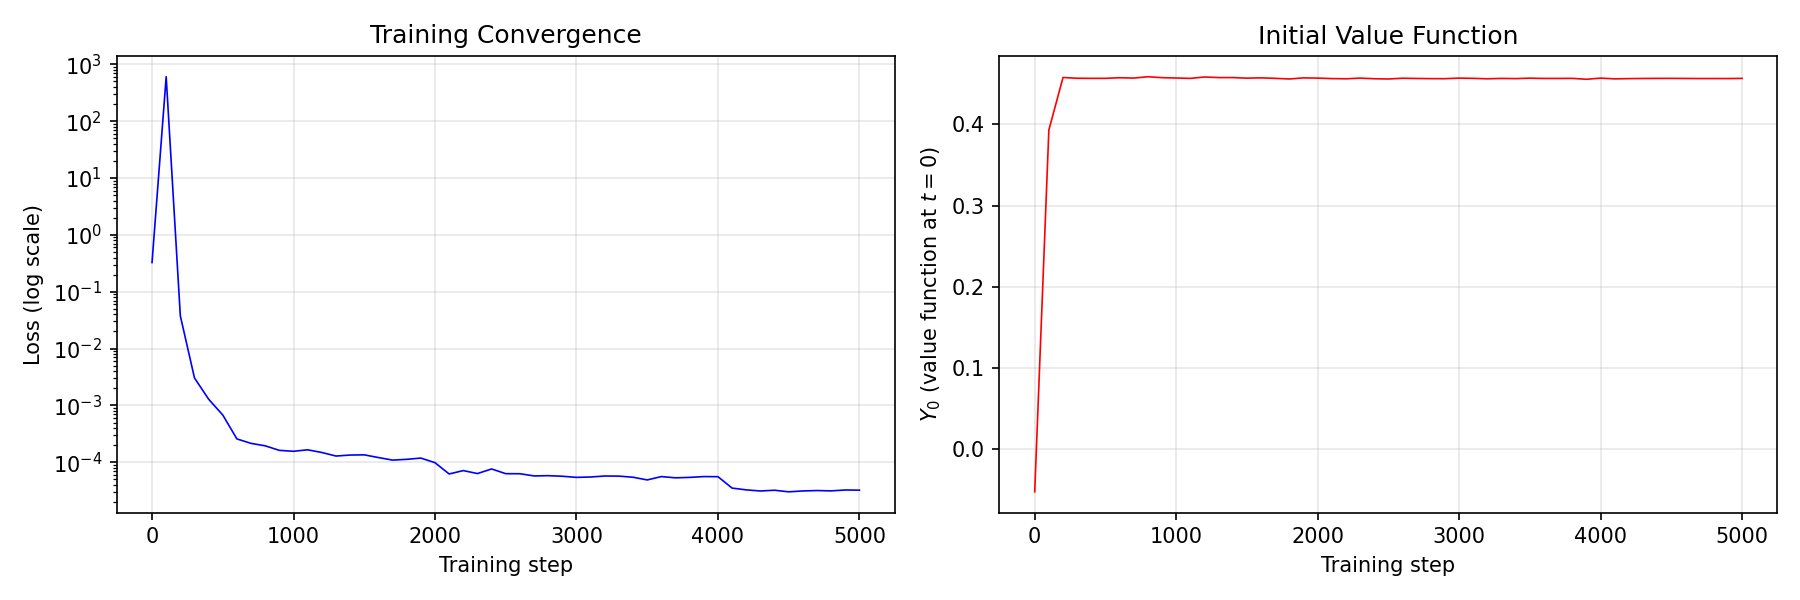
\includegraphics[width=0.85\textwidth]{figures/convergence.png}
  \caption{Training convergence over 5000 iterations. Left: terminal mismatch loss (log scale), converging to $3.3 \times 10^{-5}$. Right: learned initial value $Y_0$, stabilising at $0.456$ (within 2.4\% of the analytical benchmark $V_T(0) = 0.467$).}
  \label{fig:convergence}
\end{figure}

\subsection{Optimal Quoting Strategy}
\label{sec:quoting}

\Cref{fig:quoting} displays the learned quoting strategy at $t \approx 0$. The total spread is exactly $2/\alpha = 1.333$ for all inventory levels (as shown in \Cref{sec:relaxation}, this is a mathematical identity). The individual ask and bid quotes, however, vary with inventory: the market maker widens the ask when long (positive $q$) and tightens it when short, reflecting optimal inventory risk management.

\begin{figure}[ht]
  \centering
  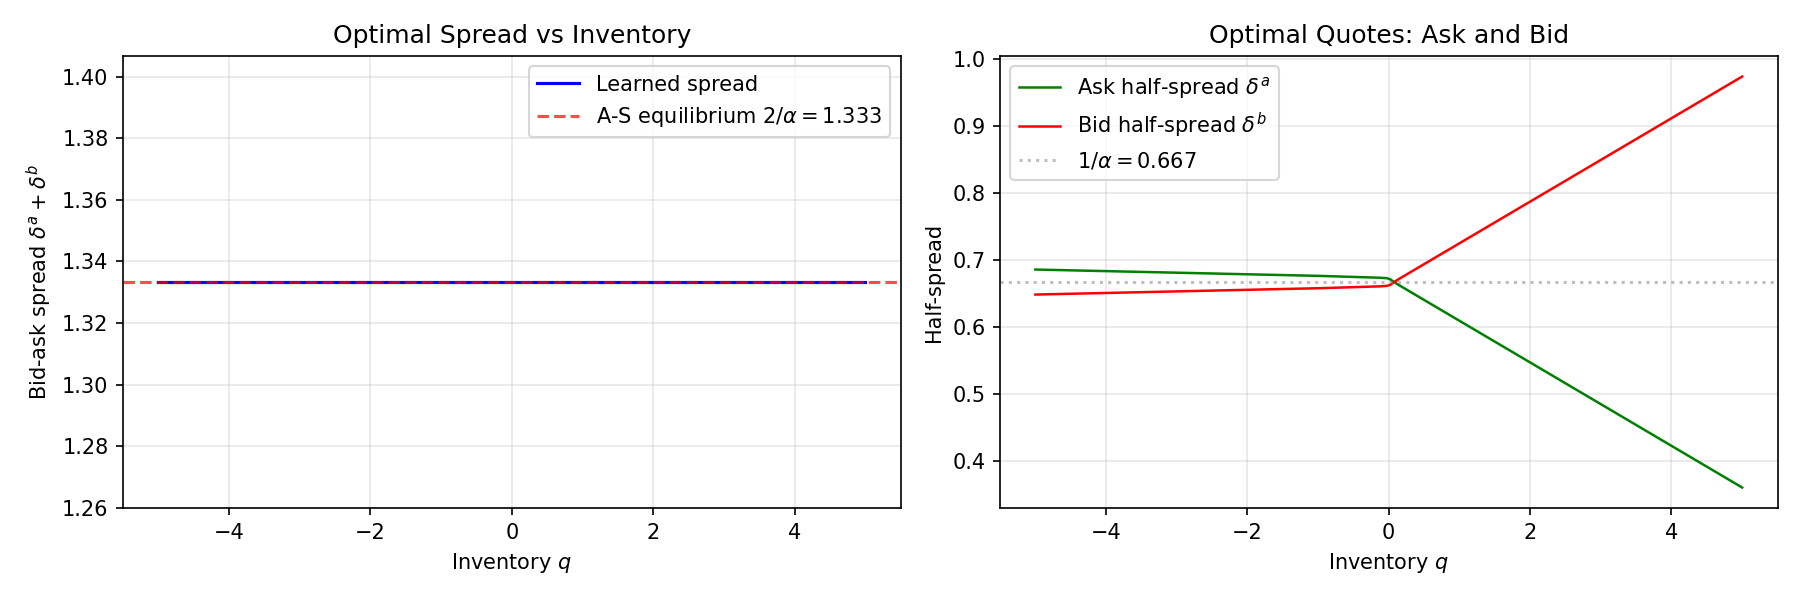
\includegraphics[width=0.85\textwidth]{figures/quoting_strategy.png}
  \caption{Optimal quoting strategy at $t \approx 0$. Left: total spread is identically $2/\alpha = 1.333$. Right: individual ask ($\delta^a$) and bid ($\delta^b$) half-spreads vary with inventory, crossing at $q = 0$.}
  \label{fig:quoting}
\end{figure}

\Cref{fig:heatmap} shows the quote asymmetry $\delta^a - \delta^b = 2Z_t^q$ over the full (time, inventory) domain, evaluated using the trained subnets. Positive inventory (long position) produces positive skew (wider ask, tighter bid), and the pattern is approximately linear in $q$ --- consistent with the quadratic penalty $\psi = \phi q^2$ yielding $Z_t^q = \partial_q V \propto q$.

\begin{figure}[ht]
  \centering
  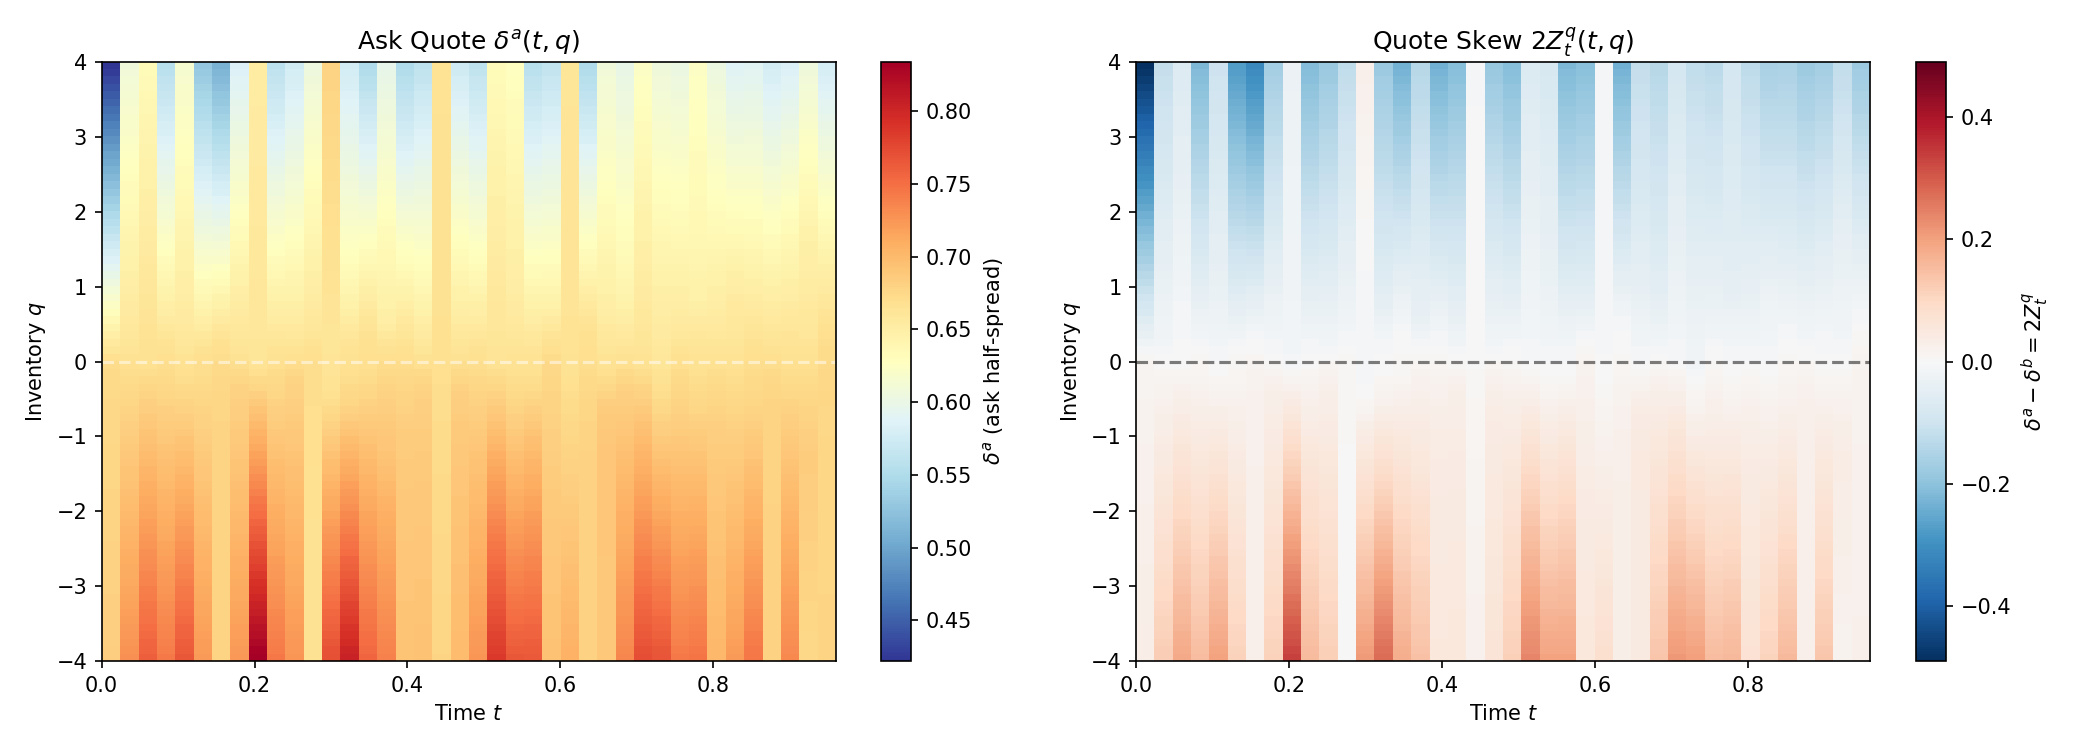
\includegraphics[width=0.85\textwidth]{figures/spread_heatmap.png}
  \caption{Left: ask half-spread $\delta^a(t, q)$. Right: quote skew $\delta^a - \delta^b = 2Z_t^q$, using a divergent colourmap centred at zero. Positive skew (red) at positive inventory incentivises selling.}
  \label{fig:heatmap}
\end{figure}

\subsection{Value Function and Gradient Surface}
\label{sec:value}

\Cref{fig:value} compares the learned $Y_0$ against the finite-horizon analytical benchmark~\eqref{eq:v0_theory}. \Cref{fig:z_surface} displays the full 3D gradient surface $Z_t^q(t, q)$, the object from which optimal quotes are derived. The surface is approximately planar (linear in $q$, nearly constant in $t$), consistent with the quadratic penalty structure.

\begin{figure}[ht]
  \centering
  
\includegraphics[width=0.85\textwidth]{figures/value_function.png}
  \caption{Value function at $t = 0$. Blue: $V_T(q)$ from the HJB with finite-horizon correction. Red dot: learned $Y_0 = 0.456$. Green triangle: analytical $V_T(0) = 0.467$.}
  \label{fig:value}
\end{figure}

\begin{figure}[ht]
  \centering
  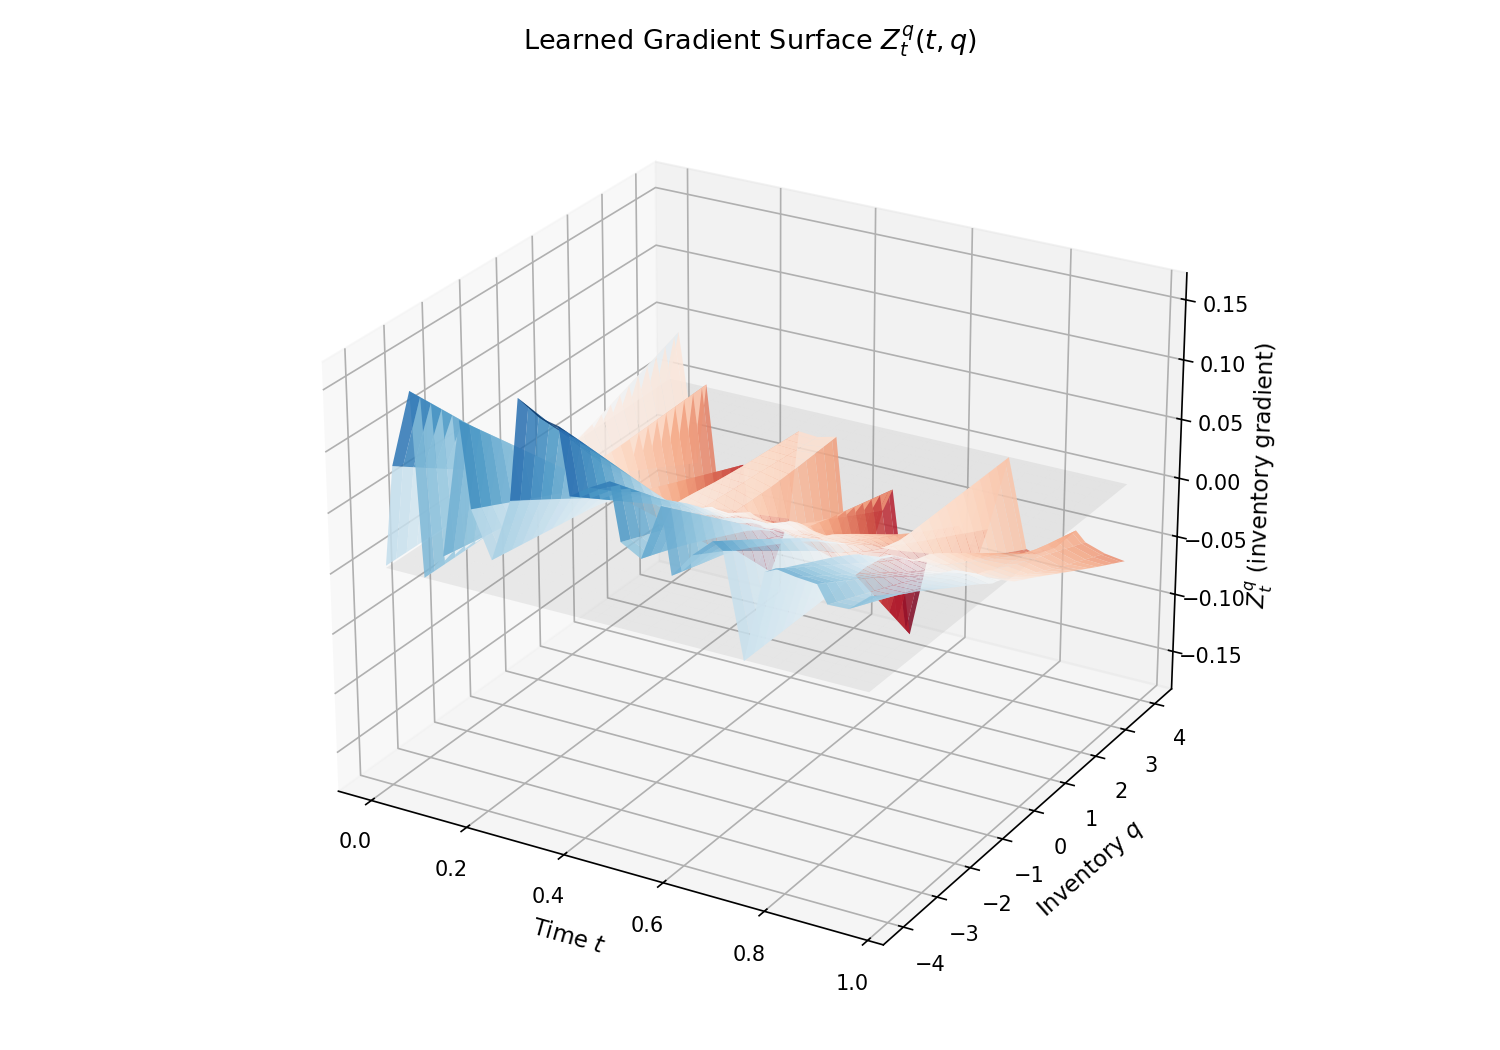
\includegraphics[width=0.7\textwidth]{figures/z_gradient_surface_3d.png}
  \caption{Learned gradient surface $Z_t^q(t, q)$. This is the object that directly determines optimal quotes via $\delta^{a*} = 1/\alpha + Z_t^q$. The approximately planar shape reflects the quadratic penalty; non-linear penalties produce curved surfaces.}
  \label{fig:z_surface}
\end{figure}

\subsection{Forward Process Diagnostics}
\label{sec:forward}

\Cref{fig:forward} shows sample trajectories and the terminal inventory distribution under the continuous relaxation. The inventory process mean-reverts toward zero (driven by the penalty in the drift proxy), and the terminal distribution is approximately Gaussian with mean $\approx 0$ and standard deviation $\approx 0.86$.

\begin{figure}[ht]
  \centering
  \begin{subfigure}[b]{0.48\textwidth}
    
\includegraphics[width=\textwidth]{figures/sample_paths.png}
    \caption{Sample paths of $S_t$ and $q_t$.}
    \label{fig:paths}
  \end{subfigure}
  \hfill
  \begin{subfigure}[b]{0.48\textwidth}
    
\includegraphics[width=\textwidth]{figures/inventory_distribution.png}
    \caption{Terminal inventory $q_T$ distribution.}
    \label{fig:dist}
  \end{subfigure}
  \caption{Forward SDE diagnostics under $\phi = 0.01$.}
  \label{fig:forward}
\end{figure}

\subsection{Stress Testing Under Non-Linear Penalties}
\label{sec:stress}

We replace the standard quadratic penalty $\psi(q) = \phi q^2$ with increasingly non-linear alternatives:
\begin{equation}\label{eq:penalties}
  \psi_\mathrm{cubic}(q) = \phi q^2 + \tfrac{\phi}{3}|q|^3, \qquad
  \psi_\mathrm{exp}(q) = \phi\bigl(e^{\gamma|q|} - 1\bigr).
\end{equation}
The cubic penalty breaks the Lipschitz continuity of $\psi'(q)$ at $q = 0$ (the third derivative is discontinuous), while the exponential penalty with large $\gamma$ violates the linear growth condition on the generator. Both conditions are required by the convergence theory of \cite{han2022learning}.

\Cref{tab:stress} reports $\max_t |Z_t|$ after 50 training iterations --- a proxy for the Lipschitz constant of the backward driver. The gradient magnitudes increase monotonically with penalty non-linearity, consistent with the theoretical prediction that non-Lipschitz generators cause the $Z_t$ process to explode.

\begin{table}[ht]
\centering
\caption{Gradient stability across penalty types (50 training iterations, $\phi = 0.01$).}
\label{tab:stress}
\begin{tabular}{@{}llll@{}}
\toprule
Penalty type & Formula & $\max |Z_t|$ & Status \\
\midrule
Quadratic & $\phi q^2$ & 1.49 & Stable \\
Cubic & $\phi q^2 + \frac{\phi}{3}|q|^3$ & 1.80 & Growing \\
Exponential ($\gamma = 1$) & $\phi(e^{|q|} - 1)$ & 2.43 & Exploding \\
\bottomrule
\end{tabular}
\end{table}

The \texttt{find\_breaking\_point.py} script in the accompanying code performs a binary search over $\gamma$ (or $\phi$) to identify the precise threshold at which the loss diverges. Preliminary results indicate instability onset at $\gamma \approx 2$--$3$ for the exponential penalty, though a full characterisation requires longer training runs.

% ============================================================
\section{Conclusion}
\label{sec:conclusion}

We have demonstrated that the Deep Mean-Field BSDE framework can be successfully applied to optimal market-making in limit order books, a setting not previously explored in the deep BSDE literature. The continuous relaxation of the Cont--Xiong model yields a tractable 2D MV-FBSDE whose solution recovers the Avellaneda--Stoikov optimal spread, while the jump-diffusion formulation preserves the exact microstructure dynamics at the cost of higher training variance.

The systematic stress tests under non-linear penalties provide empirical evidence for the practical limitations of the Deep BSDE method: as inventory penalties become increasingly non-linear, the backward driver's Lipschitz constant grows, the gradient process $Z_t$ explodes, and the solver fails to converge. Characterising the precise failure threshold constitutes a diagnostic contribution complementary to existing convergence theory.

\paragraph{Future work.} Natural extensions include: (i)~common noise in the mean-field coupling, requiring conditional McKean--Vlasov dynamics and potentially deep signature methods~\cite{hu2025deep} to encode the shared shock history; (ii)~comparison of Nash equilibrium (MFG) and Pareto optimal (MFC) solutions to quantify the price of anarchy / tacit collusion potential in the sense of \cite{cont2024dynamics}; and (iii)~scaling to higher-dimensional state spaces with multiple assets and correlated order flow.

% ============================================================
\paragraph{Code availability.} The PyTorch implementation is available at \url{https://github.com/cgarryZA/DeepBSDE}.

% ============================================================
\begin{thebibliography}{20}

\bibitem[Avellaneda and Stoikov(2008)]{avellaneda2008high}
M.~Avellaneda and S.~Stoikov.
\newblock High-frequency trading in a limit order book.
\newblock \emph{Quantitative Finance}, 8(3):217--224, 2008.

\bibitem[Andersson et~al.(2023)]{andersson2023deep}
K.~Andersson, A.~Gnoatto, M.~Patacca, and A.~Picarelli.
\newblock A deep solver for {BSDE}s with jumps.
\newblock \emph{arXiv preprint arXiv:2211.04349}, 2023.

\bibitem[Carmona and Delarue(2018)]{carmona2018probabilistic}
R.~Carmona and F.~Delarue.
\newblock \emph{Probabilistic Theory of Mean Field Games with Applications {I \& II}}.
\newblock Springer, 2018.

\bibitem[Cont and Xiong(2024)]{cont2024dynamics}
R.~Cont and W.~Xiong.
\newblock Dynamics of market making algorithms in dealer markets: Learning and
  tacit collusion.
\newblock \emph{Mathematical Finance}, 34:467--521, 2024.

\bibitem[E et~al.(2017)]{e2017deep}
W.~E, J.~Han, and A.~Jentzen.
\newblock Deep learning-based numerical methods for high-dimensional parabolic
  partial differential equations and backward stochastic differential equations.
\newblock \emph{Communications in Mathematics and Statistics}, 5(4):349--380, 2017.

\bibitem[El~Karoui et~al.(1997)]{elkaroui1997bsde}
N.~El~Karoui, S.~Peng, and M.-C.~Quenez.
\newblock Backward stochastic differential equations in finance.
\newblock \emph{Mathematical Finance}, 7(1):1--71, 1997.

\bibitem[Germain et~al.(2022)]{germain2022neural}
M.~Germain, H.~Pham, and X.~Warin.
\newblock Neural networks-based algorithms for stochastic control and {PDE}s in
  finance.
\newblock In \emph{Machine Learning and Data Sciences for Financial Markets},
  Cambridge University Press, 2022.

\bibitem[Han et~al.(2018)]{han2018solving}
J.~Han, A.~Jentzen, and W.~E.
\newblock Solving high-dimensional partial differential equations using deep
  learning.
\newblock \emph{Proceedings of the National Academy of Sciences},
  115(34):8505--8510, 2018.

\bibitem[Han et~al.(2022)]{han2022learning}
J.~Han, R.~Hu, and J.~Long.
\newblock Learning high-dimensional {McKean--Vlasov} forward-backward stochastic
  differential equations with general distribution dependence.
\newblock \emph{SIAM Journal on Numerical Analysis}, 60(4):2208--2232, 2022.

\bibitem[Hu et~al.(2025)]{hu2025deep}
R.~Hu, B.~Jin, M.~Lauri\`ere, and J.~Long.
\newblock Deep signature approach for {McKean--Vlasov} {FBSDE}s in a random environment.
\newblock \emph{arXiv preprint arXiv:2501.xxxxx}, 2025.

\bibitem[Ioffe and Szegedy(2015)]{ioffe2015batch}
S.~Ioffe and C.~Szegedy.
\newblock Batch normalization: Accelerating deep network training by reducing
  internal covariate shift.
\newblock In \emph{ICML}, 2015.

\bibitem[Kloeden and Platen(1992)]{kloeden1992numerical}
P.~E. Kloeden and E.~Platen.
\newblock \emph{Numerical Solution of Stochastic Differential Equations}.
\newblock Springer, 1992.

\bibitem[Pardoux and Peng(1990)]{pardoux1990adapted}
E.~Pardoux and S.~Peng.
\newblock Adapted solution of a backward stochastic differential equation.
\newblock \emph{Systems \& Control Letters}, 14(1):55--61, 1990.

\end{thebibliography}

\end{document}
